\textbf{PUT the examples right in the place where it is mentioned in the theory.!} 
"As we have seen in section 2.1.1.... and in section 2.2.2......"

In this first analysis, we rely on 

This analysis relies on \texttt{1inter\_stationary.R} code from the \textbf{/Scripts-R/} folder of the github repository.

This analysis relies on 2Nonstationary.R and 2NeuralsNets.R code from the\textbf{ /Scripts-
R/} folder of the github repository. A few results of nonstationary analysis in a POT approach are
presented in Section 4.1 of the \textbf{Summary1\_intro} files in the \textbf{/vignettes} folder of the repository. 

TABLE with nested models (gumbel, GEV, + linear trend, etc etc)


The block-length selection an important issue of the analysis. It is important to choose a block-length which is large enough for the limiting arguments supporting the GEV approximation (see (\ref{exttheom})) to be valid, either a large bias in the estimates could occur. For example, if this is too short, the maxima may be too close of each other to assume independence. But a large block-length implies less data to work with, and thus a large variance of the estimates. A compromise must be found between bias and variance and as pointed out in \hyperref[sec::1]{Chapter \textbf{\ref{sec::1}}}, yearly blocks seem justifiable not only for this reason (difficult to study?) but especially for their interpretability and ease of use.
\textbf{However, we will "relax" the independence assumption and present the stationary analysis in the next section. It will not change our analysis.}

\addcontentsline{toc}{subsection}{R packages for EVT}
\subsubsection*{R packages in EVT}

A plenty of packages exist for modelling extreme values in R. We have explored most of them and we used some to do the following analysis. We made comparisons and the results are the same for similar methods. Regarding the classic EVT analysis, we must name the following : 
\vspace*{-.2cm}
\begin{itemize}
	\item[$\blacktriangleright$] \texttt{ismev}, \texttt{evd}, \texttt{extRemes} (good for a wide nonstationary analysis with POT and nice tutorials, see e.g. \citet{gilleland_extremes_2016}), \texttt{ POT} (see \citet{ribatet_users_2006})\texttt{evir} \texttt{fExtremes}, $\dots$
\end{itemize}

Whereas lots of the package are doing the same analysis but with different tools, we decided to rely mostly on \texttt{ismev} as it is the package used in the book of \citet{coles_introduction_2001}.

\section{First Estimation of the Model}

Whereas the whole content of \hyperref[sec::1]{Chapter \textbf{\ref{sec::1}}} is important to understand the concepts used in this section, we will now be mostly based on inferential methods discussed in \hyperref[sec::gevinfernce]{Section\textbf{ \ref{sec::gevinfernce}}}

\subsection*{Maximum Likelihood}\label{sec:mlepratic}

Relying on the R packages cited above ,but also by checking it manually, i.e. by numerically solving the optimization problem, that is minimizing the negative log-likelihood, with the \texttt{nlm} routine using a Newton-Raphson algorithm (originated from \citet{dennis_numerical_1987}). This is based on approximating the log-likelihood by a quadratic function, the second order Taylor series approximation of the log-likelihood for a given point.  The results are shown in Table \ref{tab:estlik} :
\vspace{-.1cm}
\begin{table}[!htbp] \centering 
	\caption{Maximum likelihood estimation of the three GEV parameters} 
		\vspace{-.2cm}
	\label{tab:estlik} 
	\begin{tabular}{@{\extracolsep{5pt}} cccc} 
		\\[-1.8ex]\hline 
		\hline  \\[-1.8ex] 
		& Location $\mu$ & Scale $\sigma$ & Shape $\xi$ \\ 
		\hline \\[-1.8ex] 
		Estimates (s.e.) & $30.587$ ($0.216$)& $2.081$ ($0.155$) & $\boldsymbol{-0.254}$ ($0.067$) \\ 
		\hline \\[-1.8ex] 
	\end{tabular} 
\end{table} 
\vspace{-.2cm}

From this table \ref{tab:estlik}, an important thing to note is the value of the \textbf{shape} parameter which is negative which means that we are under a Weibull-type distribution  From figure \ref{gev3plot} this means that the density distribution has the form of the red line, i.e. having a .
Moreover, we confirmed that by doing a likelihood ratio test comparing this distribution with a Gumbel distribution. We obtained a p-value of $10^{-3}$ leading to a rejection of the Gumbel hypothesis. This obviously implies rejection of the Fréchet distribution.

The Weibull-type implies that the distribution have an estimated right endpoint given by $\hat{x}_*=\hat{\mu}-\hat{\sigma}\cdot\hat{\xi}^{-1}=38.77$. Comparing this value with the maximum value of the series (=36.6) tells us that the sample properties of this model take into account the uncertainty, from the fact that there are only 116 years of data. Hence, it allows to go beyond this maximum value, with very small probability. This is also highlighted in figure \ref{fig:rl_empdes} (right plot) where we remark that there are still probabiliy mass beyond the minimum and the maximum values of the series.

\paragraph*{Profile log-likelihood intervals} 
As discussed in \hyperref[sec:g]{Section \textbf{\ref{sec::gevinfernce}}}, \emph{profile likelihood intervals} are preferred for individual parameters to handle the poor normal approximation of the MLE. We let the results in Figure \ref{fig:proflikpar} in \hyperref[app:fig]{Appendix \textbf{\ref{app:fig}}}, provided by the \texttt{ismev} package.
These intervals are constructed in the following way : Search for the horizontal line and then subtracting the maximum log-likelihood by half the corresponding upper quantile of the $\chi^2_{\text{df}}$ for the $\text{df}=1$ parameter of interest. We notice that :
\begin{itemize}
	\item Even at $99\%$, the interval for $\hat{\xi}$ does not contain 0 supporting our statement that the distribution is left heavy-tailed and right bounded.
	\item The intervals do not present much asymetries. In fact, this will be more relevant for return levels as we will see in the \hyperref[sec:rlemp]{next Section}.
\end{itemize}


\subsection*{Probability-Weighted-Moments}

It is always a good practice to check if different methods would lead to significantly different results.
The second estimator we have seen is the \emph{probability-weighted-moments}. Results are shown in Table \ref{tab:estpwm}.

\vspace{-.1cm}
\begin{table}[!htbp] \centering 
	\caption{GEV parameters estimated by PWM} 
		\vspace{-.2cm}
	\label{tab:estpwm} 
	\begin{tabular}{@{\extracolsep{5pt}} cccc} 
		\\[-1.8ex]\hline 
		\hline  \\[-1.8ex] 
		& Location $\mu$ & Scale $\sigma$ & Shape $\xi$ \\ 
		\hline \\[-1.8ex] 
		Estimates & $30.552$ & $2.115$ & $\boldsymbol{-0.232}$ \\ 
		\hline \\[-1.8ex] 
	\end{tabular} 
\end{table} 
\vspace{-.2cm}

We directly see that these results are very close to the estimates of Table \ref{tab:estlik}, in particular for the EVI. This is encouraging for further inference, and we have hence confidence to be under a Weibull-type
model. For convenience, we will only keep the maximum likelihood estimates to work with in the following.


\subsection{Return Levels}\label{sec:rlemp}

First presented in \hyperref[rlgev]{Section \textbf{\ref{rlgev}}}, return levels are a very appreciate tool by the practitioners for inference in EVT in an environmental context.
We saw that usual likelihood intervals relying on the normal approximation are often not reliable for
return levels. Hence, we decided to compute the profile likelihood intervals and compare both values.


\vspace{-.1cm}
\begin{table}[!htbp] \centering 
	\caption{m-year return level estimates and $95\%$ intervals. Last line computes the difference between the length of the normal interval with the length of the profile likelihood interval} 
	\vspace{-.2cm}
	\label{tab:rl1} 
	\begin{tabular}{@{\extracolsep{5pt}} ccccc} 
		\\[-1.8ex]\hline 
		\hline  \\[-1.8ex] 
		&  $2$-year & $10$-year & $100$-year & $1000$-year  \\
		\hline \\[-1ex]
		\textbf{Estimates}&$ 31.315$ & $34.153$ & $36.229$ & $37.982$ \\
		 Normal interval & $(30.88, 31.75)$ & $(33.63, 34.67)$ & $(35.21, 37.25)$ & $(35.67, 39.04)$\\ 
	    Profile likelihood interval & $(31.16, 31.68)$ & $(33.95, 34.74)$ & $(35.54, 37.84)$ & $(36.58, 40.25)$  \\
		\textbf{Difference of lengths} & $0.348$ & $0.247$& $-0.260$ & $-0.294$ \\ 
		\hline \\[-1.8ex] 
	\end{tabular} 
\end{table} 
\vspace{-.2cm}

The interpretation we can make from Table \ref{tab:rl1} is that, for example, $36.23^{\circ} c$ is the temperature which will be exceeded on average once every 100 years. Note that very long term extrapolation should be tempered by caution since we only have 116 years of data and predicting far beyond this value will
be unreliable. We clearly see the shift of the profile likelihood confidence intervals compared with the
normal intervals. This can also be seen on the return level plot of Figure \ref{fig:rl_empdes} where we clearly see blue points going higher than red lines for higher values of the return period. Moreover, we see that the profile likelihood intervals are more precise\footnote{In the sense of a narrower confidence interval. A Monte-Carlo study of accuracy could be made using observed data.} 1 for "small" return periods, that is approximatively until half the total number of annual data, and then profile likelihood intervals become larger. This shows how profile likelihood intervals takes more into account the uncertainty of predicting in a far future.
Hence, in addition to arguments already provided, uncertainty but also climate warming lead us to
have preference for profile likelihood intervals. A bit surprisingly, this method is not used by default in EV packages such as \texttt{ismev}.



\subsection{Diagnostics}

\hyperref[sec:diag]{Section \textbf{\ref{sec:diag}}} provided us tools to check the accuracy of the fitted model. The goal is to check that the
model $\hat{F}$ fitted by MLE is accurate enough for the true model $F$ which is estimated by the empirical df
(\ref{eq:emprdist}). First, we present the quantile and the probability plots in Figure \ref{fig:ppqqplot}.

\begin{figure}[!htb]
	\centering	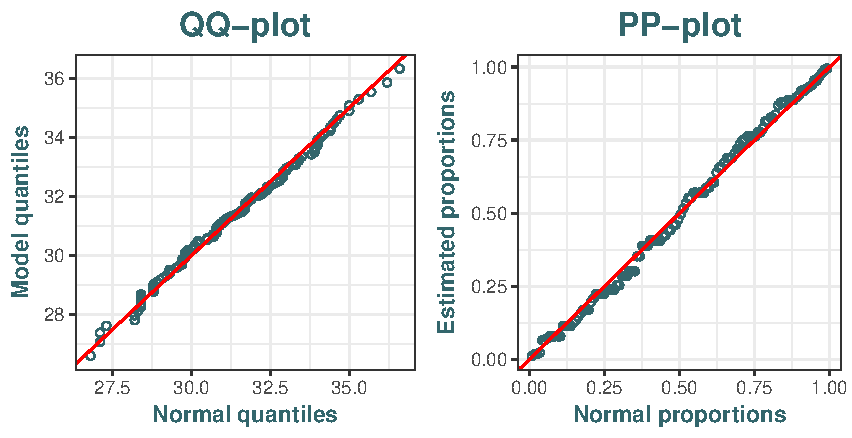
\includegraphics[width=.7\linewidth]{pp_qqplot.pdf}\caption{Quantile (left) and probability (right) plot for the stationary GEV model fitted by MLE.}\label{fig:ppqqplot}
\end{figure}

Both plots show points lying very close to the unit diagonal showing that the empirical distribution
is very close to the fitted model and hence putting confidence that our model fits our data accurately.
Right plot of Figure \ref{fig:rl_empdes} has the same interpretation and leads to the same conclusion.

\begin{figure}[!htb]
	\centering	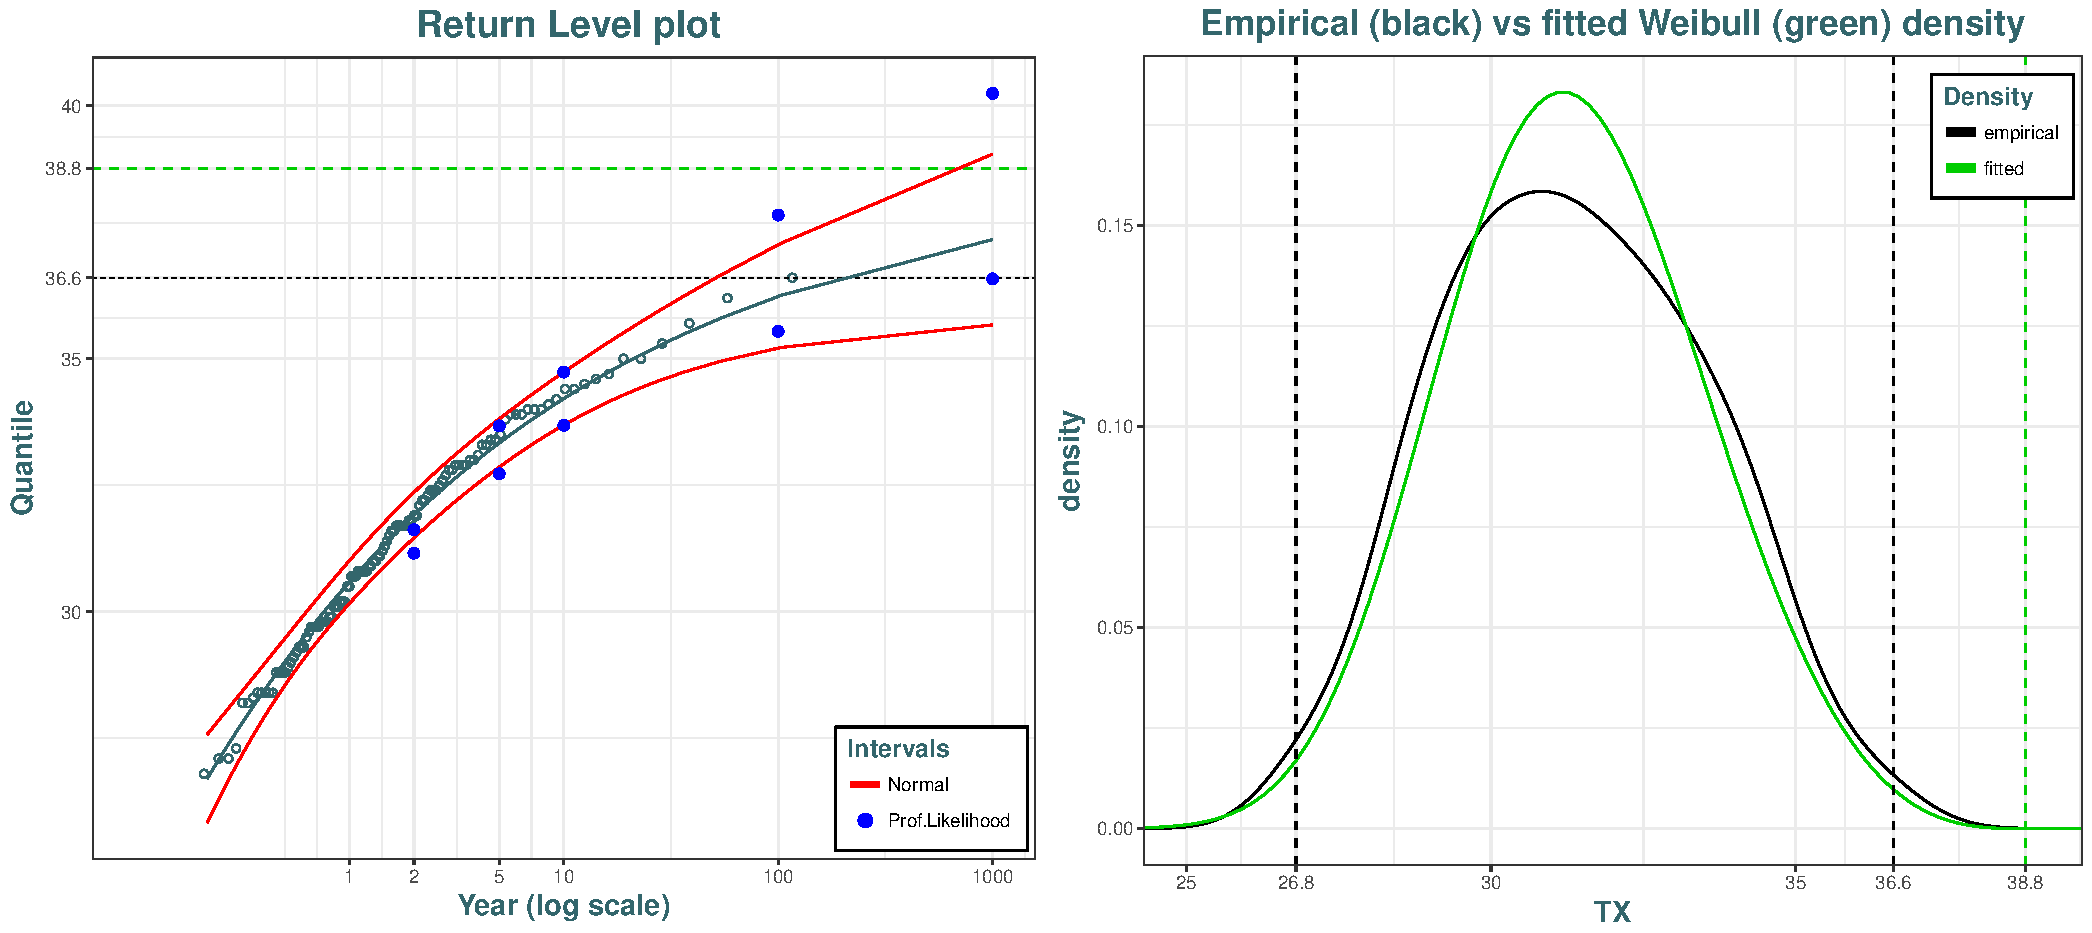
\includegraphics[width=.75\linewidth]{rl_empdes.pdf}\caption{(Left) Return level plot with red lines representing normal confidence intervals and blue points are individual profile likelihood intervals for return levels, and horizontal dotted line represent the right endpoint of the	fitted model. (Right) kernel density in blue compared with density plot of the fitted model in red, with left and right	vertical dotted lines represent respectively the minimum and maximum value of the yearly maxima series.}\label{fig:rl_empdes}
\end{figure}


\subsection*{Return Level Plot}

Another tool is available in EVT to check the fit of a model is the return level plot. It allows to compare
observations with the return levels coming from the EV Weibull model fitted by MLE. Left plot of
Figure \ref{fig:rl_empdes} shows us a concave shape of the return levels with the return period wich asymptotes to the right endpoint $x_*$ of the fitted EV Weibull model. This comes from the fact that $\xi<0$. We remark
that all points are very close the estimated return level and hence we put confidence that our model
is suitable. Moreover, all these points are inside the normal confidence intervals (and recall that profile
likelihood intervals are not suitable for very small return periods).

Whereas the estimated return level cannot go beyond $x_*$, we see that for very high return periods, the upper bound of the confidence intervals goes beyond this right endpoint. Again, this is justified since for such far periods, these intervals allow to go beyond the domain of the fitted distribution.



\subsection*{Profile Likelihood Intervals for Return Levels}

We let in \hyperref[app:fig]{Appendix \textbf{\ref{app:fig} }} the Figure \ref{fig:proflikrl} representing the profile log-likelihoods for three return periods and their corresponding intervals, that is at the intersection between the blue line and the curve. We
clearly visualize the asymmetries on these graphs and the positive skew which is increasing for higher
values of the return period. This was expected since the data at hand provide increasingly weaker
information about high levels of the process. We also displayed on the different plots the return levels
from Table \ref{tab:rl1}, represented by the green lines. These were computed relying on another method from
package \texttt{extRemes}. Results are slightly different for the $2$-year return level.


\section{Stationary Analysis}

In \hyperref[sec:statio]{Section \textbf{\ref{sec:statio}}} we have proven that when a sequence is not independent we can still have the GEV
distribution in the limit of the normalized sequence. This will only induce different location and scale
parameters compared to an independent sequence. Actually, the estimates shown in Table \ref{tab:estlik} already take this "possible" dependence into account.


\section{Nonstationary Analysis}


\subsection{Statistical Tools : Model Comparisons}

In order to compare our models, that is for example to check whether a trend is statistically significant, or if the nonstationnary models provide an improvement over the simpler (stationary) model, we will make use of the \textbf{deviance statistic} defined as 
\begin{equation}
D = 2\big\{\ell_1(\mathcal{M}_1)-\ell_0(\mathcal{M}_0)\big\},
\end{equation}

for two nested models $\mathcal{M}_0\subset \mathcal{M}_1$, where $\ell_1(\mathcal{M}_1)$ and $\ell_0(\mathcal{M}_0)$ are the maximized log-likelihoods under models $\mathcal{M}_1$ and $\mathcal{M}_0$ respectively as defined in .
Asymptotically, the distribution of $D$ is $\chi_k$ with $k$ (df) representing the difference of parameters between model $\mathcal{M}_1$ and $\mathcal{M}_0$. Thus, comparisons of $D$ with the critical values from $\chi_k$ will guide our decision.



\section{Improvements with Neural Networks}



\section{Comments and Comparisons with POT}

In practical analysis of extreme values such data, there are plenty of ways to analyze and we considered
some of them.

First of all, the other approach we have seen is in Chapitre 2 is the POT

As we did not have any precise goal to achieve, we decided to only consider the annual analysis in
block maxima.

In excess over a threshold models, the Point Process approach